\documentclass[times,specification,annotation]{itmo-student-thesis}

%% Опции пакета:
%% - specification - если есть, генерируется задание, иначе не генерируется
%% - annotation - если есть, генерируется аннотация, иначе не генерируется
%% - times - делает все шрифтом Times New Roman, собирается с помощью xelatex
%% - languages={...} - устанавливает перечень используемых языков. По умолчанию это {english,russian}.
%%                     Последний из языков определяет текст основного документа.

%% Делает запятую в формулах более интеллектуальной, например:
%% $1,5x$ будет читаться как полтора икса, а не один запятая пять иксов.
%% Однако если написать $1, 5x$, то все будет как прежде.
\usepackage{icomma}

%% Один из пакетов, позволяющий делать таблицы на всю ширину текста.
\usepackage{tabularx}

%% Данные пакеты необязательны к использованию в бакалаврских/магистерских
%% Они нужны для иллюстративных целей
%% Начало
\usepackage{tikz}
\usetikzlibrary{arrows}
\usepackage{filecontents}
\begin{filecontents}{bachelor-thesis.bib}
@online{ doerr-doerr-lambda-lambda-self-adjustment-arxiv,
    year        = {2015},
    title       = {Optimal Parameter Choices Through Self-Adjustment: Applying the 1/5-th Rule in
                   Discrete Settings},
    author      = {Benjamin Doerr and Carola Doerr},
    url         = {http://arxiv.org/abs/1504.03212},
    year        = {2015},
    langid      = {english}
}

@inproceedings{ example-english,
    year        = {2015},
    booktitle   = {Proceedings of IEEE Congress on Evolutionary Computation},
    author      = {Maxim Buzdalov and Anatoly Shalyto},
    title       = {Hard Test Generation for Augmenting Path Maximum Flow 
                   Algorithms using Genetic Algorithms: Revisited},
    pages       = {2121-2128},
    langid      = {english}
}

@article{ example-russian,
    author      = {Максим Викторович Буздалов},
    title       = {Генерация тестов для олимпиадных задач по программированию 
                   с использованием генетических алгоритмов},
    journal     = {Научно-технический вестник {СПбГУ} {ИТМО}},
    number      = {2(72)},
    year        = {2011},
    pages       = {72-77},
    langid      = {russian}
}

@article{ unrestricted-jump-evco,
    author      = {Maxim Buzdalov and Benjamin Doerr and Mikhail Kever},
    title       = {The Unrestricted Black-Box Complexity of Jump Functions},
    journal     = {Evolutionary Computation},
    year        = {2016},
    note        = {Accepted for publication},
    langid      = {english}
}

@book{ bellman,
    author      = {R. E. Bellman},
    title       = {Dynamic Programming},
    address     = {Princeton, NJ},
    publisher   = {Princeton University Press},
    numpages    = {342},
    pagetotal   = {342},
    year        = {1957},
    langid      = {english}
}
\end{filecontents}
%% Конец

%% Указываем файл с библиографией.
\addbibresource{bachelor-thesis.bib}

\begin{document}

\studygroup{M3439}
\title{Распознавание новообразований по КТ изображениям легких}
\author{Крючков Максим Игоревич}{}Крючков М.И.}
\supervisor{Фильченков Андрей Александрович}{Фильченков А.А.}{к.ф-м.н.}{Научный сотрудник Университета ИТМО}
\publishyear{2020}
%% Дата выдачи задания. Можно не указывать, тогда надо будет заполнить от руки.
\startdate{01}{сентября}{2019}
%% Срок сдачи студентом работы. Можно не указывать, тогда надо будет заполнить от руки.
\finishdate{31}{мая}{2020}
%% Дата защиты. Можно не указывать, тогда надо будет заполнить от руки.
\defencedate{15}{июня}{2020}

\addconsultant{Ефимова В.А.}{без звания}

\secretary{Павлова О.Н.}

%% Задание
%%% Техническое задание и исходные данные к работе
\technicalspec{Требуется разработать стилевой файл для системы \LaTeX, позволяющий оформлять бакалаврские работы и магистерские диссертации
на кафедре компьютерных технологий Университета ИТМО. Стилевой файл должен генерировать титульную страницу пояснительной записки,
задание, аннотацию и содержательную часть пояснительной записк. Первые три документа должны максимально близко соответствовать шаблонам документов,
принятым в настоящий момент на кафедре, в то время как содержательная часть должна максимально близко соответствовать ГОСТ~7.0.11-2011
на диссертацию.}

%%% Содержание выпускной квалификационной работы (перечень подлежащих разработке вопросов)
\plannedcontents{Пояснительная записка должна демонстрировать использование наиболее типичных конструкций, возникающих при составлении
пояснительной записки (перечисления, рисунки, таблицы, листинги, псевдокод), при этом должна быть составлена так, что демонстрируется
корректность работы стилевого файла. В частности, записка должна содержать не менее двух приложений (для демонстрации нумерации рисунков и таблиц
по приложениям согласно ГОСТ) и не менее десяти элементов нумерованного перечисления первого уровня вложенности (для демонстрации корректности
используемого при нумерации набора русских букв).}

%%% Исходные материалы и пособия 
\plannedsources{\begin{enumerate}
    \item ГОСТ~7.0.11-2011 <<Диссертация и автореферат диссертации>>;
    \item С.М. Львовский. Набор и верстка в системе \LaTeX;
    \item предыдущий комплект стилевых файлов, использовавшийся на кафедре компьютерных технологий.
\end{enumerate}}

%%% Цель исследования
\researchaim{Разработка удобного стилевого файла \LaTeX
             для бакалавров и магистров кафедры компьютерных технологий.}

%%% Задачи, решаемые в ВКР
\researchtargets{\begin{enumerate}
    \item обеспечение соответствия титульной страницы, задания и аннотации шаблонам, принятым в настоящее время на кафедре;
    \item обеспечение соответствия содержательной части пояснительной записки требованиям ГОСТ~7.0.11-2011 <<Диссертация и автореферат диссертации>>;
    \item обеспечение относительного удобства в использовании~--- указание данных об авторе и научном руководителе один раз и в одном месте, автоматический подсчет числа тех или иных источников.
\end{enumerate}}

%%% Использование современных пакетов компьютерных программ и технологий
\addadvancedsoftware{Пакет \texttt{tabularx} для чуть более продвинутых таблиц}{\ref{sec:tables}, Приложения~\ref{sec:app:1}, \ref{sec:app:2}}
\addadvancedsoftware{Пакет \texttt{biblatex} и программное средство \texttt{biber}}{Список использованных источников}

%%% Краткая характеристика полученных результатов 
\researchsummary{Получился, надо сказать, практически неплохой стилевик. В 2015--2018 годах
его уже использовали некоторые бакалавры и магистры. Надеюсь на продолжение.}

%%% Гранты, полученные при выполнении работы 
\researchfunding{Автор разрабатывал этот стилевик исключительно за свой счет и на
добровольных началах. Однако значительная его часть была бы невозможна, если бы
автор не написал в свое время кандидатскую диссертацию в \LaTeX,
а также не отвечал за формирование кучи научно-технических отчетов по гранту,
известному как <<5-в-100>>, что происходило при государственной финансовой поддержке
ведущих университетов Российской Федерации (субсидия 074-U01).}

%%% Наличие публикаций и выступлений на конференциях по теме выпускной работы
\researchpublications{По теме этой работы я (к счастью!) ничего не публиковал.
\begin{refsection}
Однако покажу, как можно ссылаться на свои публикации из списка литературы:
\nocite{example-english, example-russian}
\printannobibliography
\end{refsection}
}

%% Эта команда генерирует титульный лист и аннотацию.
\maketitle{Бакалавр}

%% Оглавление
\tableofcontents

%% Макрос для введения. Совместим со старым стилевиком.
\startprefacepage

В данном разделе размещается введение.


Из всех раковых заболеваний рак легких наиболее рапространен по всему миру. Более того на данный момент он является одним из самых тяжелых раковых заболеваний по показателям смертности. В связи с этим задача распознавания новообразований по КТ изображениям легких очень актуальна, поскольку эффективные методы поиска новообразований способствуют диагностике заболеваний на ранней стадии, что позволяет своевременно назначить лечение и в конечном счете сократить число летальных исходов.

Трехмерные сканы легких, полученные с помощью компьютерной томографии могут могут содержать до $512 \times 512 \times 600$ вокселов. При этом в основном диаметр опухоли составляет не более 30mm (среднее значение диаметра новообразований в датасете LIDC-IDRI \cite{lidc} равняется 15 мм). Каждый воксел в среднем эквивалентен от 0.7 до 2 мм по каждой из пространственных осей, что свидетельствует о том, что опухоли невелики по сравнению со всем изображением. 

Маленькие размеры опухолей, отсутствие некоторого 



%% Начало содержательной части.
\chapter{Обзор предметной области}

%% Так помечается начало обзора.
\startrelatedwork
\section{Сверточные нейронные сети}

\section{ResNet}

\section{Squeeze and Excitation}

Squeeze and Excitation (SE)

Модуль SE был предложен в 2017 году и показала SOTA результат в соревновании ImageNet. Данный модуль, который предполагается включать в сеть после каждого сверточного блока, позволяет использовать зависимости между различными каналами блока и масштабировать с помощью вектора коэффициентов, обучаемых в отдельной маленькой сети (какой??) 

[картинка]


\section{Генеративные противоборствующие сети}


\section{Адаптивная нормализация объектов}

Адаптивная нормализация объектов - технология нормализации выходов внутренних слоев сети, которая была предложена в работе[] для совершенствования модели переноса стиля одного изображения на другое

Это афинное преобразование входа $x$ параметризованное некоторым $y$:

$$AdaIN(x, y) = \sigma(y)(\dfrac{x - \mu(x)}{\sigma(x)}) + \mu(y)$$

Авторы предполагали использовать стиль в качестве $y$, однако в последствии данную нормализацию стали применять.

В области генеративных противоборствующих сетей AdaIN можно применять не только для решения задачи переноса стиля, но и для обучения эффективных параметров нормализации. В роли $y$ может выступать выход некоторой побочной сети, принимающей на вход латентный вектор.
Пример ссылок в рамках обзора: \cite{example-english, example-russian, unrestricted-jump-evco, doerr-doerr-lambda-lambda-self-adjustment-arxiv}.
%% Так помечается конец обзора.
\finishrelatedwork
Вне обзора:~\cite{bellman}.

\chapter{Описание предлагаемого подхода для 2D сегментации}

\section{Распространенный подход}

Было проведено множество исследований в области сегментации КТ изображений легких. Одним из основных подходов является двухшаговая модель, где на первом этапе локализуется предполагаемый 3D участок, содержащий опухоль (Volume of Interest, VOI), а на втором этапе производится непосредственная сегментация внутри выбранного участка. Интуитивное объяснение данной модели состоит в том, что пространство, занимаемое опухолью, достаточно мало по сравнению со всем КТ изображением.

\section{Предлагаемый подход}

Однако было предложено использовать другую модель, производящую сегментацию изображения end-to-end. Данная модель показала отличный результат (первое место) в соревновании Data Science Bowl 2018. В последствии модель была применена к другой задаче - сегментации глиальных опухолей головного мозга по данным МРТ, где показала хороший результат.

Архитектура модели включает очень глубокую encoder-decoder сверточную сеть типа Unet. Также модель использует комбинированную функцию потерь, состоящую из кросс-энтропии наряду с мягкой функцией потерь Дайса. Ожидалось, что модель способна показать хороший результат и в задаче сегментации КТ легких.

На рисунке \ref{mri-sample} визуализирована работа сети на изображении МРТ.

\begin{figure}[!h]
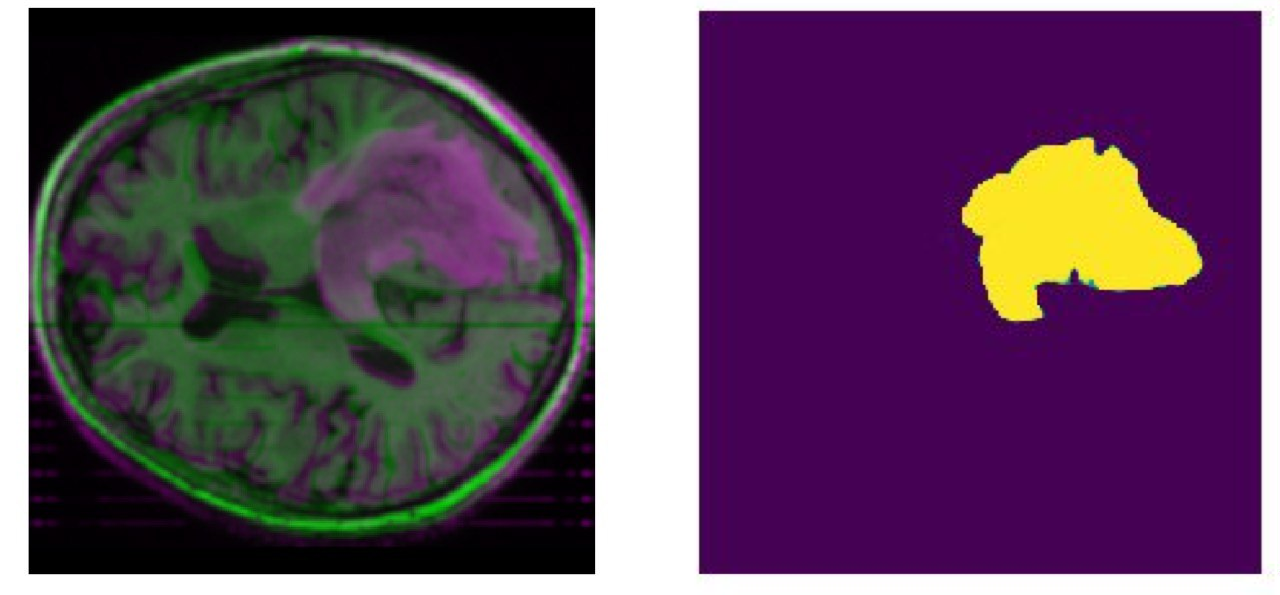
\includegraphics[width=\linewidth]{images/mri-sample.png}
\caption{Пример работы сети на изображении МРТ}\label{mri-sample}
\centering
\end{figure}

\chapter{Описание предлагаемого подхода для 3D локализации}

В этой главе будут описан предлагаемое решение задачи 3D локализации новообразований по снимкам КТ легких.

\section{Модель локализации опухолей}

Для детекции опухолей была заимстована сверточная сеть с архитектурой Squeeze and Excitation Encoder Decoder \cite{deep-seed}. Сеть использует архитектуру ResNet18 в качестве кодировщика со встроенными SE модулями после каждого сверточного блока ResNet (остаточного блока). 

Структуру кодировщика отражает декодирощик, слои которого связаны skip-соединениями с кодировщиком. Выход декодирвщика подается на вход Region Proposal Network (RPN), задачей которой является предсказание координат различных bounding box-ов и вероятностей того, что в том или ином bounding box-е заключено новообразование.

\begin{figure}[!h]
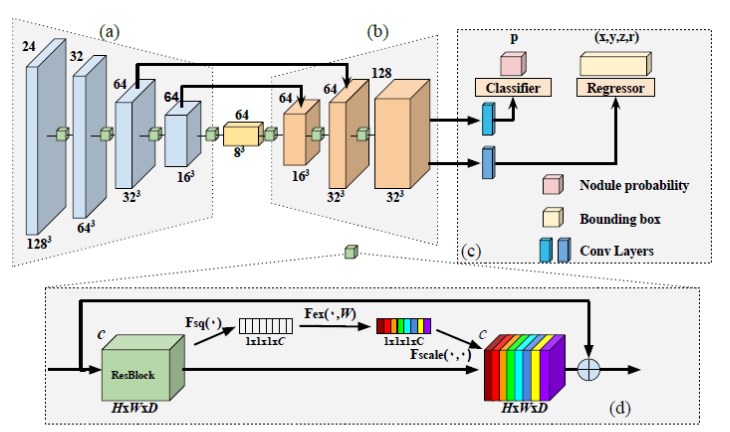
\includegraphics[width=\linewidth]{deep-seed-architecture.png}
\caption{Архитектура используемой сети DeepSEED}\label{deep-seed-architecture}
\centering
\end{figure}


\section{Аугментация данных с помощью генеративных противоборствующих сетей}

Широко известно применение генератиных противоборствующих сетей для генерации данных, которые впоследствии могут быть использованы в качестве расширения существующего датасета, на котором предполагается обучать детектор. В ряде работ были проведены визуальные тесты Тьюринга, где радиологам было предложено попробовать отличить генерированные опухоли от оригинальных. Специалисты не очень хорошо справились с задачей, что может говорить о том, что сети способны генерировать достаточно хорошие изображения, чтобы их можно было использовать в обучающем множестве.

\subsection{Модель генеративной противоборствующей сети}

Для решения данной задачи было принято решение заимствовать сеть, предложенную в работе \cite{mirsky}. У данной статьи есть документированная и удобная реализация в открытом доступе, в которой реализованы два фреймворка - один предназначен для добавления генерированных опухолей на изображение, второй предназначем для удаления опухолей с изображения. Для задачи аугментации данных естественно позаимствовать первый фреймворк который помимо реализации непосредственно архитектуры сети, предоставляет еще и возможность предобработки данных, которая состоит из нормализации и гистограммного выравнивания изображений.

Модель построена на условных GAN (Conditional GAN, CGAN), и основной задачей генератора является создание правдоподобной опухоли из некоторого шума и контекста. Сеть получает на вход $x_r^*$ - участок КТ изображения размера $32^3$, содержащий опухоль, из которого вырезан центральный куб размера $16^3$, и на его место вставлена маска из нулей. Оставшаяся часть участка $x_r^*$ выступает в роли контекстного окружения. Сеть генератора состоит из нескольких сверточных слоев (кодировщика) и нескольких декодирующих слоев, которые соединены с кодирующими слоями попарно (skip connection). После каждого сверточного блока применяется батчевая нормализация. Выход генератора - $G(x_r^*, \theta_g)$ наряду с оригинальным участком изображения $x_r$ далее подаются на вход дискриминатору, задачей которого является классифицировать объекты как оригинальные или генерированные.

\begin{figure}[!h]
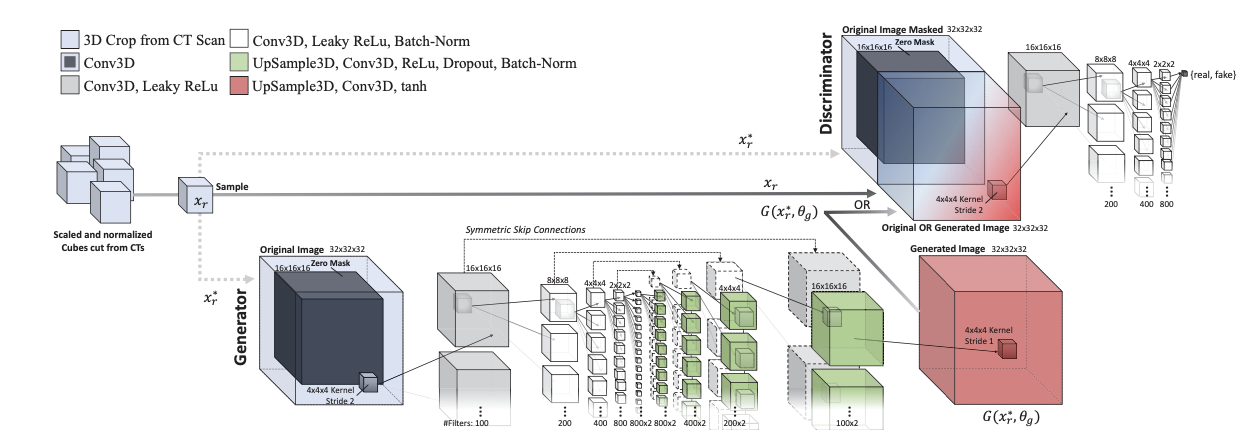
\includegraphics[width=\linewidth]{mirskiy-cgan-architecture.png}
\caption{Архитектура используемой сети CGAN}\label{mirskiy-cgan-architecture}
\centering
\end{figure}

\subsection{Адаптивная нормализация объектов (AdaIN)}

Адаптивная нормализация является популярной технологией и служит альтернативой батчевой нормализации и объектной нормализации, применяемой после каждого сверточного блока. Поэтому для совершенствования генеративной сети было предложено использовать ее вместо батчевой нормализации для эффективного и обучаемого преобразования промежуточных данных.

Адаптивная нормализация применяется следующим образом: Тензором $x$ принимается на вход. Размерности тензора: 

$$(b, xdim, ydim, zdim, c)$$, где $b$ - количество объектов в батче, $c$ - количество каналов, $xdim, ydim, zdim$ - пространственные размерности сооответственно.

нормализуется по все пространственным измерениям, то есть это происходит независимо для каждого канала и объекта в отличие от батчевой нормализации и аналогично объектной нормализации (Instance Normalization). Параметры афинного преобразования имеют размерность 

$$(b, 1, 1, 1, c)$$

То есть данные параметры аналогично варьируются по каналам и объектам.

\section{Итоговая процедура обучения}

В результате предложенная процедура обучения имеет следующий вид:

\begin{enumerate}
    \item Из датасета КТ изображений легких выбираются те, которые удовлетворяют некоторым ограничениям и соответственно являются пригодными для обучения CGAN
    \item Из выбранных данных вырезанются участки, содержащие опухоль, для создания объектов, которые можно непосредственно подать на вход CGAN.
    \item Данные аугментируются стандартными способами (повороты, отражения)
    \item Данные проходят предобработку: гистограммное выравнивание и нормализацию
    \item Данные, снабженные шумом на месте опухоли и окружающим контекстом подаются на вход CGAN для обучения
    \item Сеть CGAN, натренированная генерировать опухоли получает на вход предобработанные контексты для непосредственной генерации
    \item Данные, полученные на выходе CGAN, дополняют оригинальный датасет
    \item Сеть DeepSEED обучается на дополненном датасете.
\end{enumerate}





\section{Данные}

В качестве датасета использовался LIDC-IDRI \cite{lidc} - открытый набор данных в формате DICOM, размеченный 4-мя радиологами. Всего в датасете содержится 1018 сканов и более 7000 новообразований. Новообразование включалось в размеченное множество, если оно было выявлено хотя бы одним из специалистов.


\section{Детали реализации}

\subsection{Обучение}

Изначально планировалось подавать на вход сети полные 2D изображения для того, чтобы сеть смогла получить эффективное представление признаков изображений и выявить характерные свойства пространственного расположения опухолей. Однако результат данного подхода был отрицательный, поскольку сеть была не в состоянии обучиться и функция потерь не уменьшалась. Попытки использовать другую архитектуру Unet сети и изменить функцию потерь на функцию Focal Loss, отдающую предпочтение ложно положительным пикселям нежели ложно-отрицательным, не привели к успеху. Неудачу также потерпела попытка уменьшить количество данных в обучающем множестве убрав двухмерные изображения, не содержащие опухоли вообще, которых было более 80\%.

Подобное поведение сети скорее всего объясняется тем, что градиентный спуск застрявает в локальном минимуме, который соответствует тому, что сеть выдает пустые изображения, поскольку площадь маски очень мала по сравнению с изображеним.

Чтобы решить данную проблемы было предложено подавать сети не полные изображения, а их обрезанные куски. Изображение делилось сеткой на $n^2$ равных частей, из которых выбирались две части - содержащая опухоль и не содержащая. Далее эти части подавались на вход сети. При $n = 8$ сеть все еще не могла обучиться, но при $n = 16$ удалось получить результат.

\subsection{Тестирование}

Поскольку адекватный результат сеть выдавала только на маленьких обрезанных кусках изображения, для тестирования была использована следующая стратегия:

\begin{enumerate}
    \item Изображение делилось сеткой на $16^2$ частей
    \item Каждая часть независимо подавалась на вход сети
    \item Выходы сети склеивались для получения итоговой маски
    \item Так как выход сети представляет из себя двумерный массив пикселей, где значение каждого пикселя является действительным числом, вручную выбирается некоторый порог $0 < t < 1$
    \item Все пиксели имеющие значение, большее $t$, считаются пикселями маски, остальные пиксели зануляются
\end{enumerate}



\section{Подсчет метрик качества}

Основным показателем соответствия между истинной и предсказанной маской был выбран коэффициент Дайса

$$ dice(y_{true}, y_{pred}) = \dfrac{2|y_{true} \cap y_{pred}|}{ |y_{true}| + |y_{pred}|} $$

Если модель выдавала пустую маску, и при этом в реальности на изображении не было патологий, коэффициент Дайса полагался равным $1$. Ниже приведены коэффициенты Дайса, усредненные по тестовой выборке для различных значений порога $t$ 

В качестве примера таблицы приведена таблица~\ref{tab1}.

\begin{table}[!h]
\caption{Таблица умножения (фрагмент)}\label{tab1}
\centering
\begin{tabular}{|*{18}{c|}}\hline
\textbf{Порог $t$} & \textbf{Коэффициент Дайса} \\\hline
0.4 & 0.15 \\\hline
0.45 & 0.08 \\\hline
0.5 & 0.1 \\\hline
\end{tabular}
\end{table}

\section{Визуальный анализ}

\begin{figure}[!h]
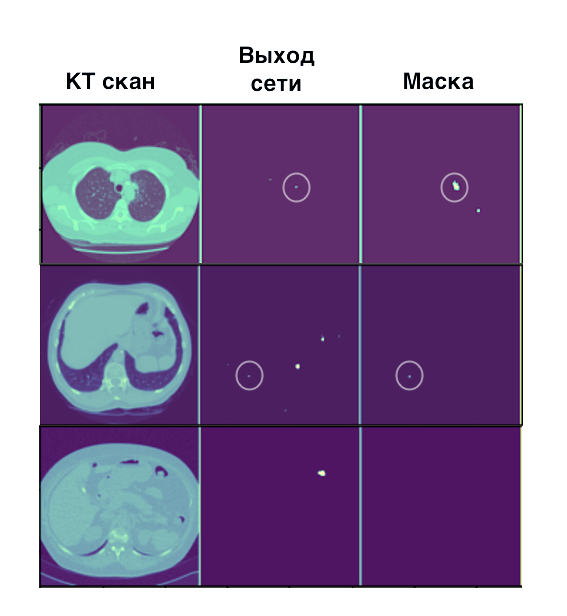
\includegraphics[width=\linewidth]{images/2d-seg-results.png}
\caption{Результаты работы сети}\label{mirskiy-cgan-architecture}
\centering
\end{figure}

Кругом обозначены совпадения на выходе сети и на истинной маске. На нижнем примере видно, что сеть ошибочно распознала участок ткани визуально похожий на опухоль, но в реальности ею не являющийся.

\section{Выводы по главе 2}

Полученные результаты явно свидетельствуют о непригодности использования подобных $end-to-end$ технологий для сегментации $2d$ изображений. Предполагаемое объяснение состоит в том, что двухмерные сканы не в состоянии передать достаточный набор признаков, позволяющий отличить опухоль от другого, похожего на нее участка легкого. Дело в том, что каждый двухмерный слайс содержит только лишь срез трехмерной опухоли, и значительная часть таких срезов может иметь вполне неопределенную форму, ничем не отличимую от сосудов в легких. Отсюда следует большая необходимость в использовании трехмерных зависимостей между различными слайсами для решения задачи распознавания.



\chapter{Результаты решения задачи 3D локализации}

\section{Используемые данные}



\section{Детали реализации}

\subsection{Реализация DeepSEED}

В оригинальной работе было предложено подавать на вход сети обрезанные участки КТ изображений размера $128^3$, однако такая размерность входных данный требует вычислительных ресурсов, которые были недоступны во время реализации, что привело к уменьшению размерности входа до $64^3$.

\subsection{Реализация CGAN}

Основная архитектура CGAN, формат и размерность входных и выходных данных были практически полностью заимствованы у авторов статьи.

\subsection{Реализация Адаптивной нормализации}

Адаптивная нормализация была добавлена в сеть вместо батчевой нормализации. Она применяется после всех блоков (свертка, активация) и в кодировщике, и в декодировщике кроме первого слоя. В качестве входа $x$ формулы $kek$ используется тензор, полученный на выходе активации, а в качестве параметра $y$ используется выход побочной сети, имеющей простую архитектуру - 3 полносвязных слоя, причем первые два разделены между всеми побочными сетями. Данная архитектура позволяет выявить эффективные параметры афинного преобразования посредством обучения.

\section{Результаты}

\subsection{Результаты локализации с помощью DeepSEED}




\chapterconclusion


%% Макрос для заключения. Совместим со старым стилевиком.
\startconclusionpage

В данном разделе размещается заключение.

\printmainbibliography


\end{document}